\section{Flächen in Kartesische Koordinaten}

\begin{itemize}
	\item\textit{Eine Fläche S ist eine \textbf{Regelfläche} falls durch jeden ihrer Punkte eine Gerade existiert, die vollständig in S liegt.}
	\item\textit{\textbf{doppelte Regelfläche} falls durch jeden ihrer Punkte zwei unterschiedliche Geraden existieren}
\end{itemize}



\textbf{Explizite Darstellung} \\
\textit{Sattel:}
$z = f(x,y) = x^2 - y^2$ \\
\\
\textbf{Implizite Darstellung} \\
\textit{Kugel:}
$(x-x_0)^2 + (y-y_0)^2 + (z-z_0)^2 = R^2$ \\
\textit{$x_0$, $y_0$, $z_0$ = Zentrum}
\\
\textbf{Parameterdarstellung} \\

Zylinderkoordinaten:
\textit{$(r,\theta,z)$}
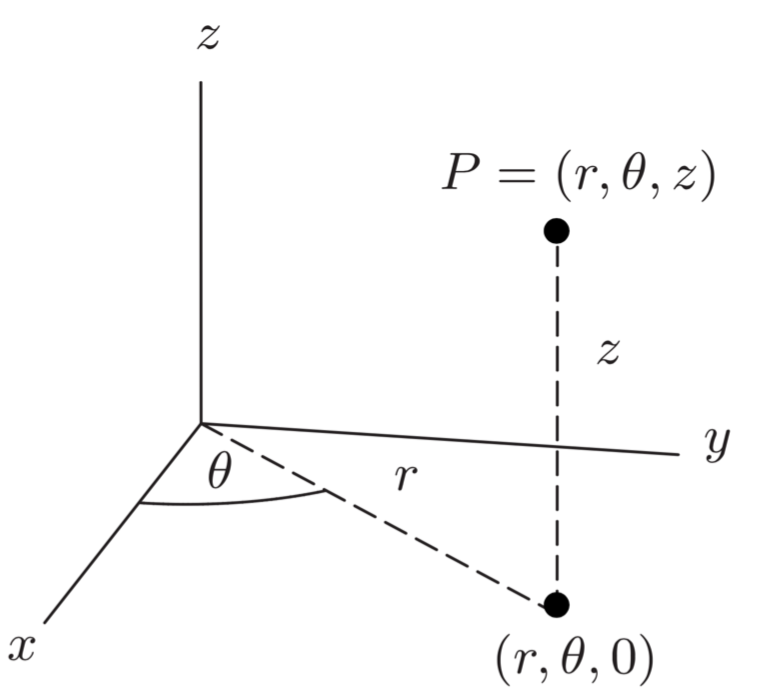
\includegraphics[width=0.3\textwidth]{assets/Zylinderkoordinaten.png}
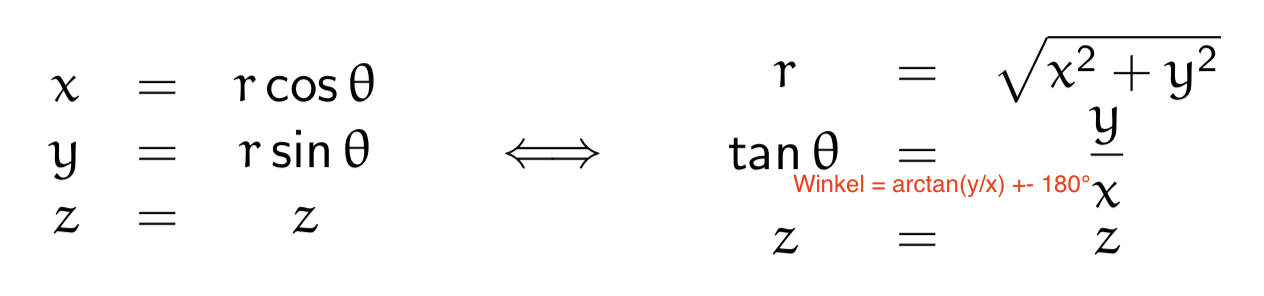
\includegraphics[width=0.4\textwidth]{assets/ZylinderkoordinatenUmrechnnung.png}

Kugelkoordinaten:
\textit{$(\rho,\phi,\theta)$}
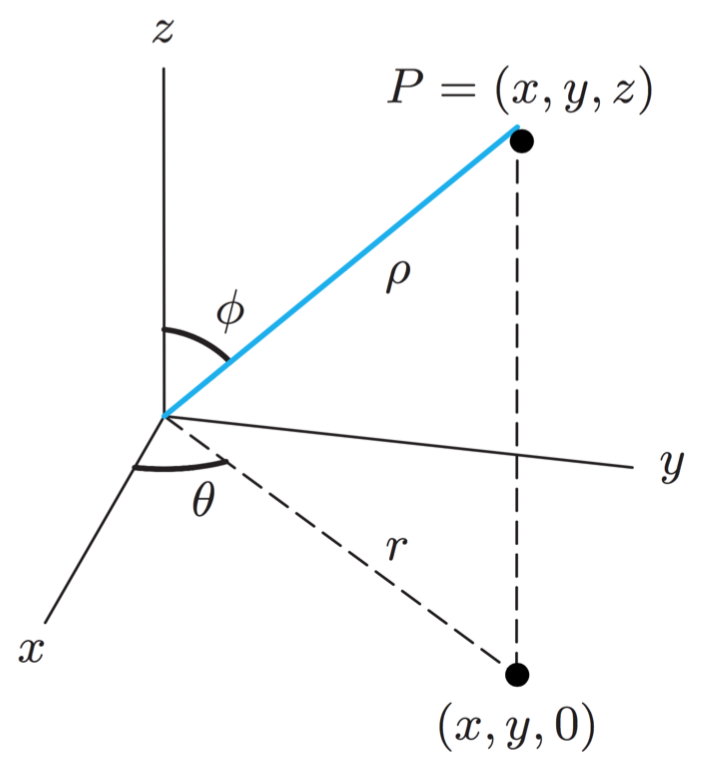
\includegraphics[width=0.3\textwidth]{assets/Kugelkoordinaten.png}
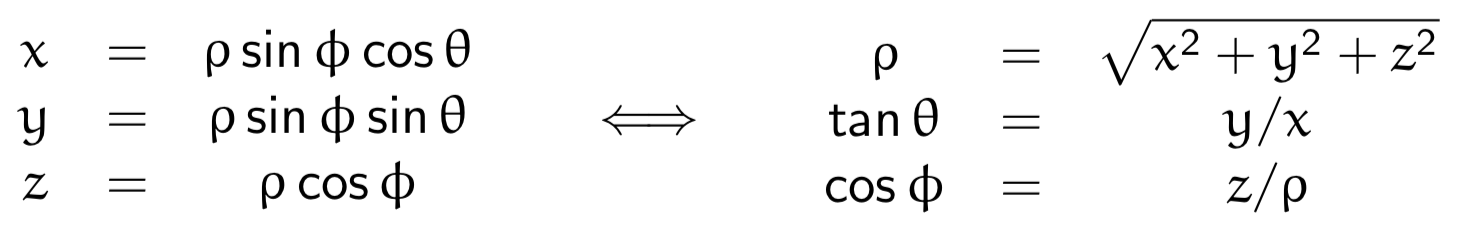
\includegraphics[width=0.4\textwidth]{assets/KugelkoordinatenUmrechnung.png}

Rotationsfläche:\\
\textit{$x=u$}\\
\textit{$y = f(x) * cos(v)$}\\
\textit{$z = f(x) * sin(v)$}\\

\subsection{Freiformflächen}

\textit{Handelt sich dabei und den selben Ansatz wie bei den Kurven,
nur auf flächen, siehe Kurven:}\\

$F(u) = \displaystyle \sum^n_{i=0}(C_i N_i (u))$, $0 \leq u \leq 1$\\
\textit{Kurve $F(u)$ mit Grad $n$}\\
$G(u) = \displaystyle \sum^m_{j=0}(C_j N_j (v))$, $0 \leq v \leq 1$\\
\textit{Kurve $G(u)$ mit Grad $m$}\\

$S(u,v) = \displaystyle \sum^n_{i=0}\sum^m_{j=0}(C_iC_jN_i(u)N_j(v))$, $0 \leq u, v \leq 1$\\
\textit{$S(u,v)$ definiert die Tensorproduktfläche}

\textit{Wobei $C_i$, $C_j$ Kontrollpunkte sind und $N_i$, $N_j$ die Splineformel}

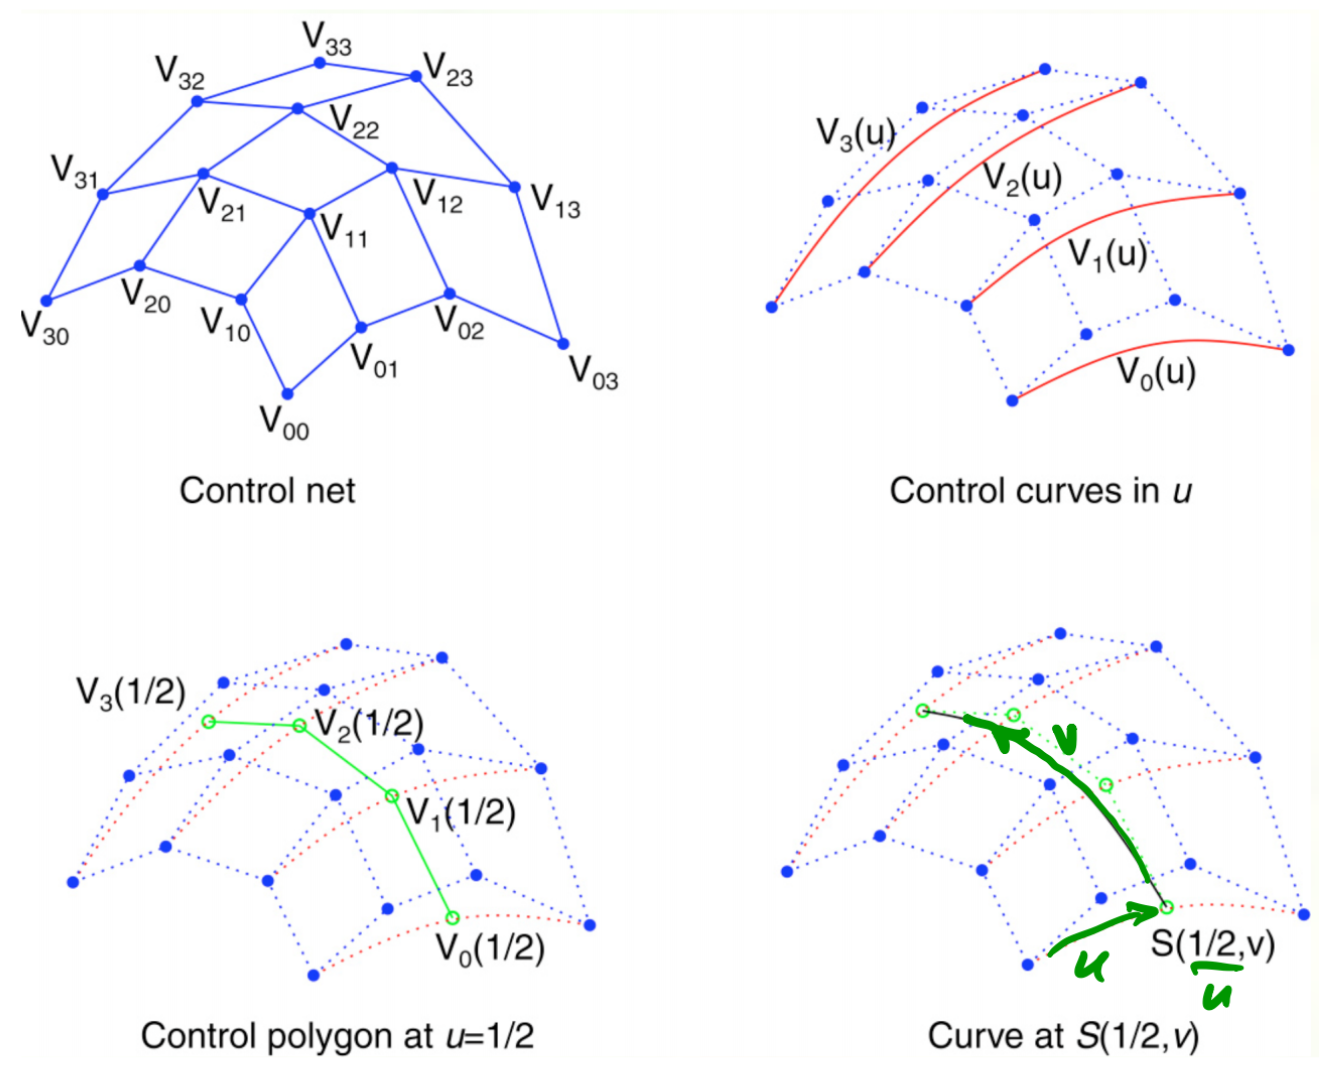
\includegraphics[width=0.5\textwidth]{assets/area-splines.png}

\begin{itemize}
	\item Tensorproduktfläche S(u,v) = Fläche gegeben von Kurven F(u) \& G(v) \\
	\textit{Für jeden u Wert gibt es eine Kurve -> "Gitterpunkte"}
\end{itemize}